\chapter{Vorgehensweise und Methodik}

\section{Themenfindung}
Die zunehmende Digitalisierung und der technologische Fortschritt eröffnen vielfältige Einsatzmöglichkeiten für Methoden der künstlichen Intelligenz (KI). Besonders im Bildungsbereich entsteht dadurch die Chance, Prozesse zu optimieren und Lehrkräfte bei Routineaufgaben zu entlasten. Vor diesem Hintergrund wurde das Thema dieser Arbeit gewählt. Ziel ist es, das Potenzial von KI-gestützten Verfahren im Kontext der automatisierten Auswertung studentischer Programmierlösungen zu untersuchen. Durch die Clusterung ähnlicher Lösungen können neue Ansätze für Feedbackprozesse entwickelt werden, die eine effizientere und gezieltere Betreuung von Studierenden ermöglichen.

\section{Recherche und Vorbereitung}
Zu Beginn wurden diverse Quellen herausgesucht, die sich im Rahmen dieses Themas bewegen. Besonders oft stach dabei der k-Means Algorithmus heraus oder wie dieser als Grundlage für erweiternde Algorithmen wie den InvAASTCluster (vgl. \cite{Orvalho.28.06.2022}) oder AsanasCluster (vgl. \cite{Paiva.2024}) benutzt wurde um bessere Ergebnisse zu liefern. Anhand eines Rankings wurde die Relevanz der Quellen festgelegt, um das weitere Vorgehen einzugrenzen. Andere Methoden wie der Caliński-Harabasz Index oder der Silhouette Score wurden erwähnt die zur Evaluation des Clusterings dienten. Es wurde klar, dass der Verlauf von studentischen Programmierlösungen bis zu nutzbaren Daten zur Feedbackgenerierung ein mehrschrittiger Prozess sein wird. Erst mit Hilfe des KI-basierten Sprachmodell-Chatbots von OpenAI (ChatGPT) wurde der Prozess bzw. die Pipeline für das Programm grob definiert. 

\section{Implementierungsverlauf}
\subsection{Erster Implementierungsabschnitt}
Durch den ersten Prototyp der Pipeline ergaben sich folgende grobe Anforderungen an das Programm:
\begin{itemize}
    \item Das Programm muss Java-Dateien einlesen können.
    \item Das Programm muss eine YAML-Konfigurationsdatei laden können.
    \item Das Programm muss für eingelesene Java-Dateien ein Embedding erstellen können.
    \item Das Programm muss Embeddings in ihren Dimensionen reduzieren können.
    \item Das Programm muss Embeddings clustern können.
    \item Das Programm muss Cluster evaluieren können.
    \item Das Programm muss Cluster visuell darstellen können.
\end{itemize}
Erst nachdem die einzelnen Prozessschritte in der Pipeline platz gefunden hatten, wurde klar welche Module dafür implementiert werden mussten. Als erstes mussten die Java-Dateien der studentischen Programmierlösugen eingelesen werden können. Diese wurden als Datensätze durch den betreuenden Prof. Dr. Striewe bereitgestellt. Der Datensatz an denen das Programm fortlaufend getestet wurde, bestand aus mehreren Überordner und final aus drei Java-Dateien und einer Text-Datei, welche den Studenten vorgegeben waren und vervollständigt werden mussten, jedoch soll die Menge der Java-Dateien keine überwiegende Rolle spielen. Das Programm musste also in der Lage sein Ordner zu durchsuchen und Java-Dateien zu erkennen. Dies ermöglichte eine Methode des ersten implementierten Moduls \texttt{data\_loader.py}. Es extrahierte Quellcode-Text unspeicherte pro Datei \texttt{code\_snippets} in eine Liste und gab diese an die Pipeline zurück. Anfgans entstanden durch problematische Zeichen innerhald der Java-Dateien Fehlermeldungen und zudem war das Modul nur daraus ausgelegt einen Ordner zu durchsuchen und nicht auch deren Unterordner. Der Code wurde auf Hinsicht der Flexibilität und Vertragbarkeit angepasst, sodass die Anzahl der Unterordner keine Rolle mehr spielte und problematische Zeichen ignoriert werden.

Als nächstes folgte das Modul zum einbetten (Embedding) dieser \texttt{code\_snippets}, um sie für das Clustering vorzubereiten. Dafür wurde das Modul \texttt{embedding\_model.py} erstellt, welches anhand einer Methode, importierte vortrainierter Sprachmodelle aus der Transformers-Bibliothek von Python (hier CodeBERT) und passende Tokenizer, die den Code vorbereitend für den Transformer in Tokens zerlegt. Zusammen werden dadurch die \texttt{code\_snippets} in numerische Vektoren umwandelt\footnote{\url{https://huggingface.co/docs/transformers}}. Das entstandene Embedding wwurde anschließend in an die Pipeline zurückgegeben und in eine Liste abgespeichert.

Nun mussten die Embeddings geclustert werden. Das entsprechend erstellte Modul \texttt{clustering\_engine.py} importierte dafür die beiden Cluster Algorithmen k-Means aus der scikit-learn Bibliothek\footnote{\url{https://scikit-learn.org/stable/modules/generated/sklearn.cluster.KMeans.html}} für machine learning und der separaten hdbscan Python-Bibliothek\footnote{\url{https://hdbscan.readthedocs.io/en/latest/api.html\#hdbscan.hdbscan.HDBSCAN}}. Das benutzte Modell wird in der Config-Datei festgelegt. An die Pipeline werden schließlich mit Markierungen (labels) versehene Cluster zurückgegeben.

Anschließend wurde ein Evaluierungsverfahren eingebaut, um die Qualität der Cluster zu bewerten. Dafür wurde das Modul \texttt{evaluation\_metrics.py} implementiert. Darin wird jeder Cluster nach den Evaluierungsverfahren Silhouette Score\footnote{\url{https://scikit-learn.org/stable/modules/generated/sklearn.metrics.silhouette_score.html}}, Caliński-Harabasz Index\footnote{\url{https://scikit-learn.org/stable/modules/generated/sklearn.metrics.calinski_harabasz_score.html}} und den Davies-Bouldin Index\footnote{\url{https://scikit-learn.org/stable/modules/generated/sklearn.metrics.davies_bouldin_score.html}} getesten, welche ebenfals aus der scikit-learn Bibliothek importiert wurden. Zurückgegeben wird ein Dictionary mit den drei Zahlenwerten der Bewertungsmetriken.

Jedes implementierte Modul wurde einzeln getestet. Dazu wurden die Ergebnisse und die Zeit, die für den jeweiligen Prozessschritt notwendig war durch print-Anweisungen ausgegeben. Dabei stellte sich heraus, dass Embedding und besonders Imports relativ viel Zeit in Anspruch nahmen. Da die zu testenden Datensätze teilweise aus mehreren hunderten Dateien bestanden, wurde dazu caching eingeführt, um das Testen des Zusammenspiels der einzelnen Module zu beschleunigen, was jedoch später wieder entfernt wurde. Versuche die Imports durch lazy loading zu beschleunigen waren in diesem Fall nur geringfügig in dem nächsten beschriebenen Schritt verwendbar. Des Weiteren wurde eine Requirements.txt-Datei erstellt. Diese beeinhaltet sämltiche Information über die aktuell im Projekt benutzen Versionen der importierten Bibliotheken. Sie sorgt, dass für andere Nutzende gleiche Bedingungen wie auch in der Entwicklung herrschen um ein lauffähiges Programm zu gewährleisten. Die noch später hinzugefügte Datei HowToInstall.txt dient dabei als Schritt-für-Schritt-Anleitung. Eine config.yaml-Datei diente als Ansprechquelle der Pipeline für Parameter 

Bevor das Visualisierungs-Modul sinnvoll eingesetzt werden konnte, wurde noch ein weiterer ProzessSchritt eingebunden, das Dimensionsreduktionsverfahren. Das entsprechende Modul \texttt{dimensionality\_reducer.py} importiert auch hier Verfahren aus der scikit-learn Bibliothek, die Principal Component Analysis (PCA)\footnote{\url{https://scikit-learn.org/stable/modules/generated/sklearn.decomposition.PCA.html}} und t-Distributed Stochastic Neighbor Embedding (t-SNE)\footnote{\url{https://scikit-learn.org/stable/modules/generated/sklearn.manifold.TSNE.html}}. Das dritte Verfahren Uniform Manifold Approximation and Projection (UMAP)\footnote{\url{https://umap-learn.readthedocs.io/en/latest/}} stammt aus der eigenständigen umap-learn Bibliothek. Dieser Prozessschritt findet zwischen Embedding und Clustering statt. Er reduziert die Embeddings bzw. Vektoren in ihren Dimensionen (hier 2D oder 3D), welche danach zur Clusterung weitergereicht werden können.

Die Pipeline besteht zu diesem Zeitpunkt aus folgendem Ablauf:
\textbf{Daten laden} $\rightarrow$ \textbf{einbetten} $\rightarrow$ \textbf{Dimensionen reduzieren} $\rightarrow$ \textbf{clustern} $\rightarrow$ \textbf{evaluieren} $\rightarrow$ \textbf{visualisieren}

Schließlich wurde noch das Modul \texttt{cluster\_plotter.py} implementiert, welches anhand der dimensions-reduzierten Embeddings und der aus dem Clustering hervorgegangenen labels ein statisches Diagramm (engl. plot) in einem separatem Fenster erstellt. Hierfür wurden aus der Matplotlibs die Plotting-Module pyplot\footnote{\url{https://matplotlib.org/stable/api/pyplot_summary.html}} und \texttt{mpl\_toolkits.mplot3d}\footnote{\url{https://matplotlib.org/stable/gallery/mplot3d/2dcollections3d.html\#sphx-glr-gallery-mplot3d-2dcollections3d-py}} importiert, die für 2D- und 3D-Visualisierung (falls gewünscht) zuständig sind. Die zuvor erstellten Module gleichten sich durch ihre einheitlichen Klassenstruktur, da jedoch für dieses Modul keine Zwischenspeicherung von Zuständen anhand einer Instanz notwendig war, wurden dessen Methoden statisch definiert, um sie direkt aufrufen zu können.

\begin{figure} %[hbtp]
	\centering
	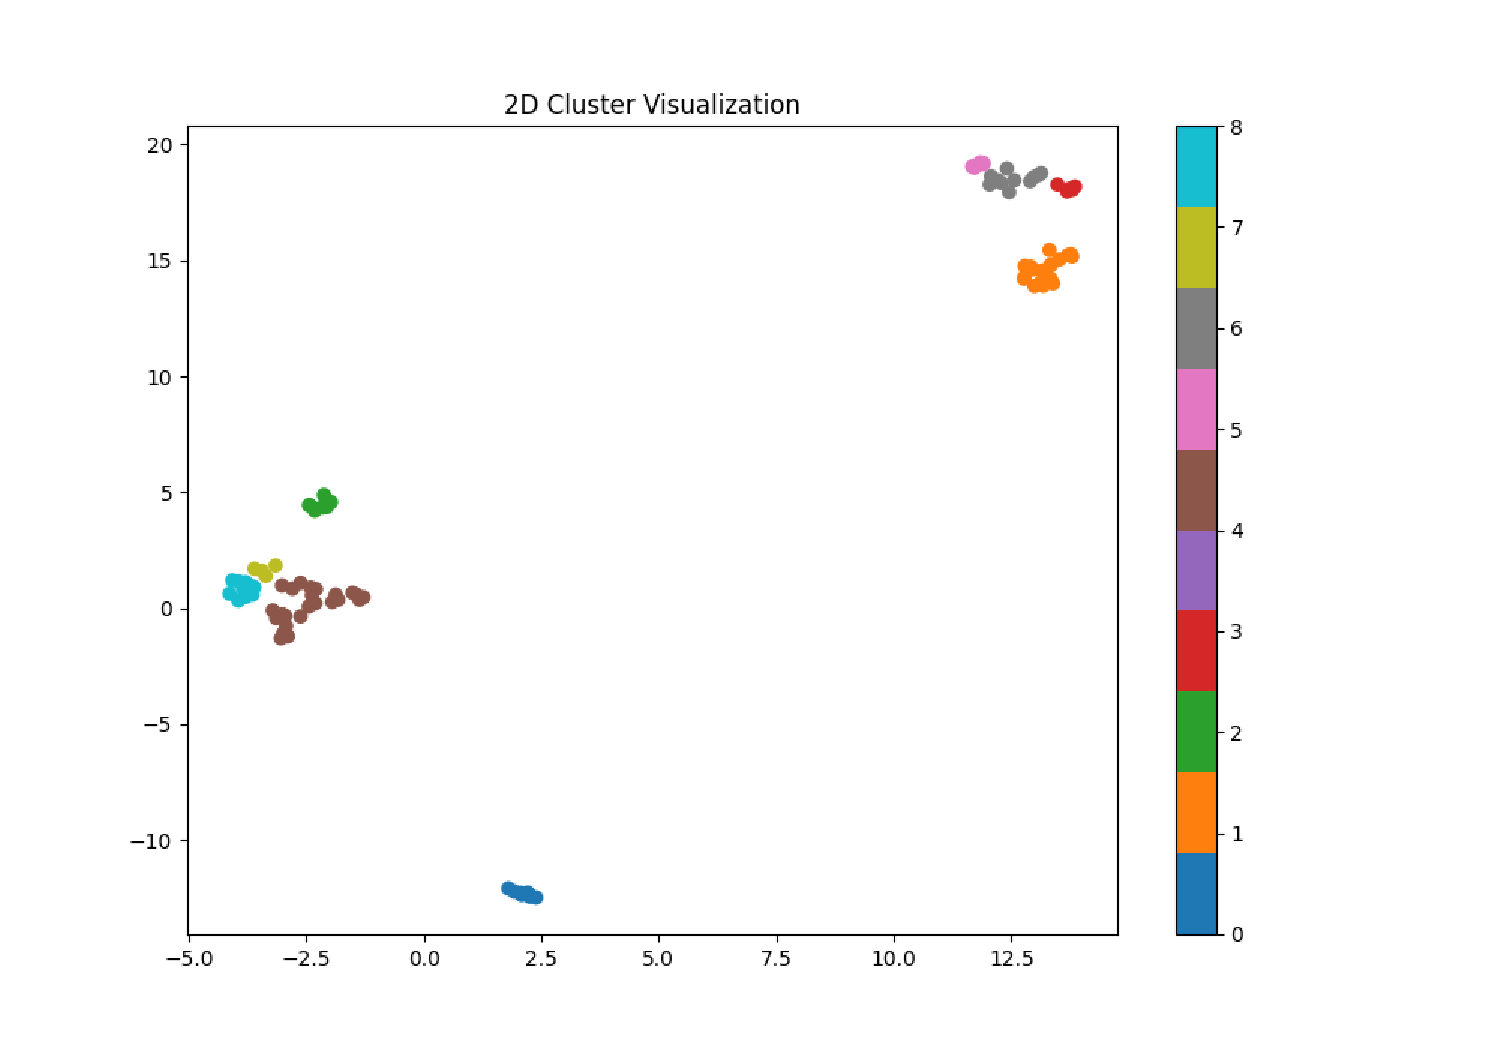
\includegraphics[width=0.8\textwidth]{images/Erstes Clustering-Diagramm.pdf}
	\caption{Clustering-Diagramm einer Clusterung von 147 Java-Dateien. Die unterschiedlichen Farben kennzeichnen die Zugehörigkeit der Punkte zu einem Cluster.}
	\label{Erstes Clustering-Diagramm}
\end{figure}

\begin{figure} %[hbtp]
	\centering
	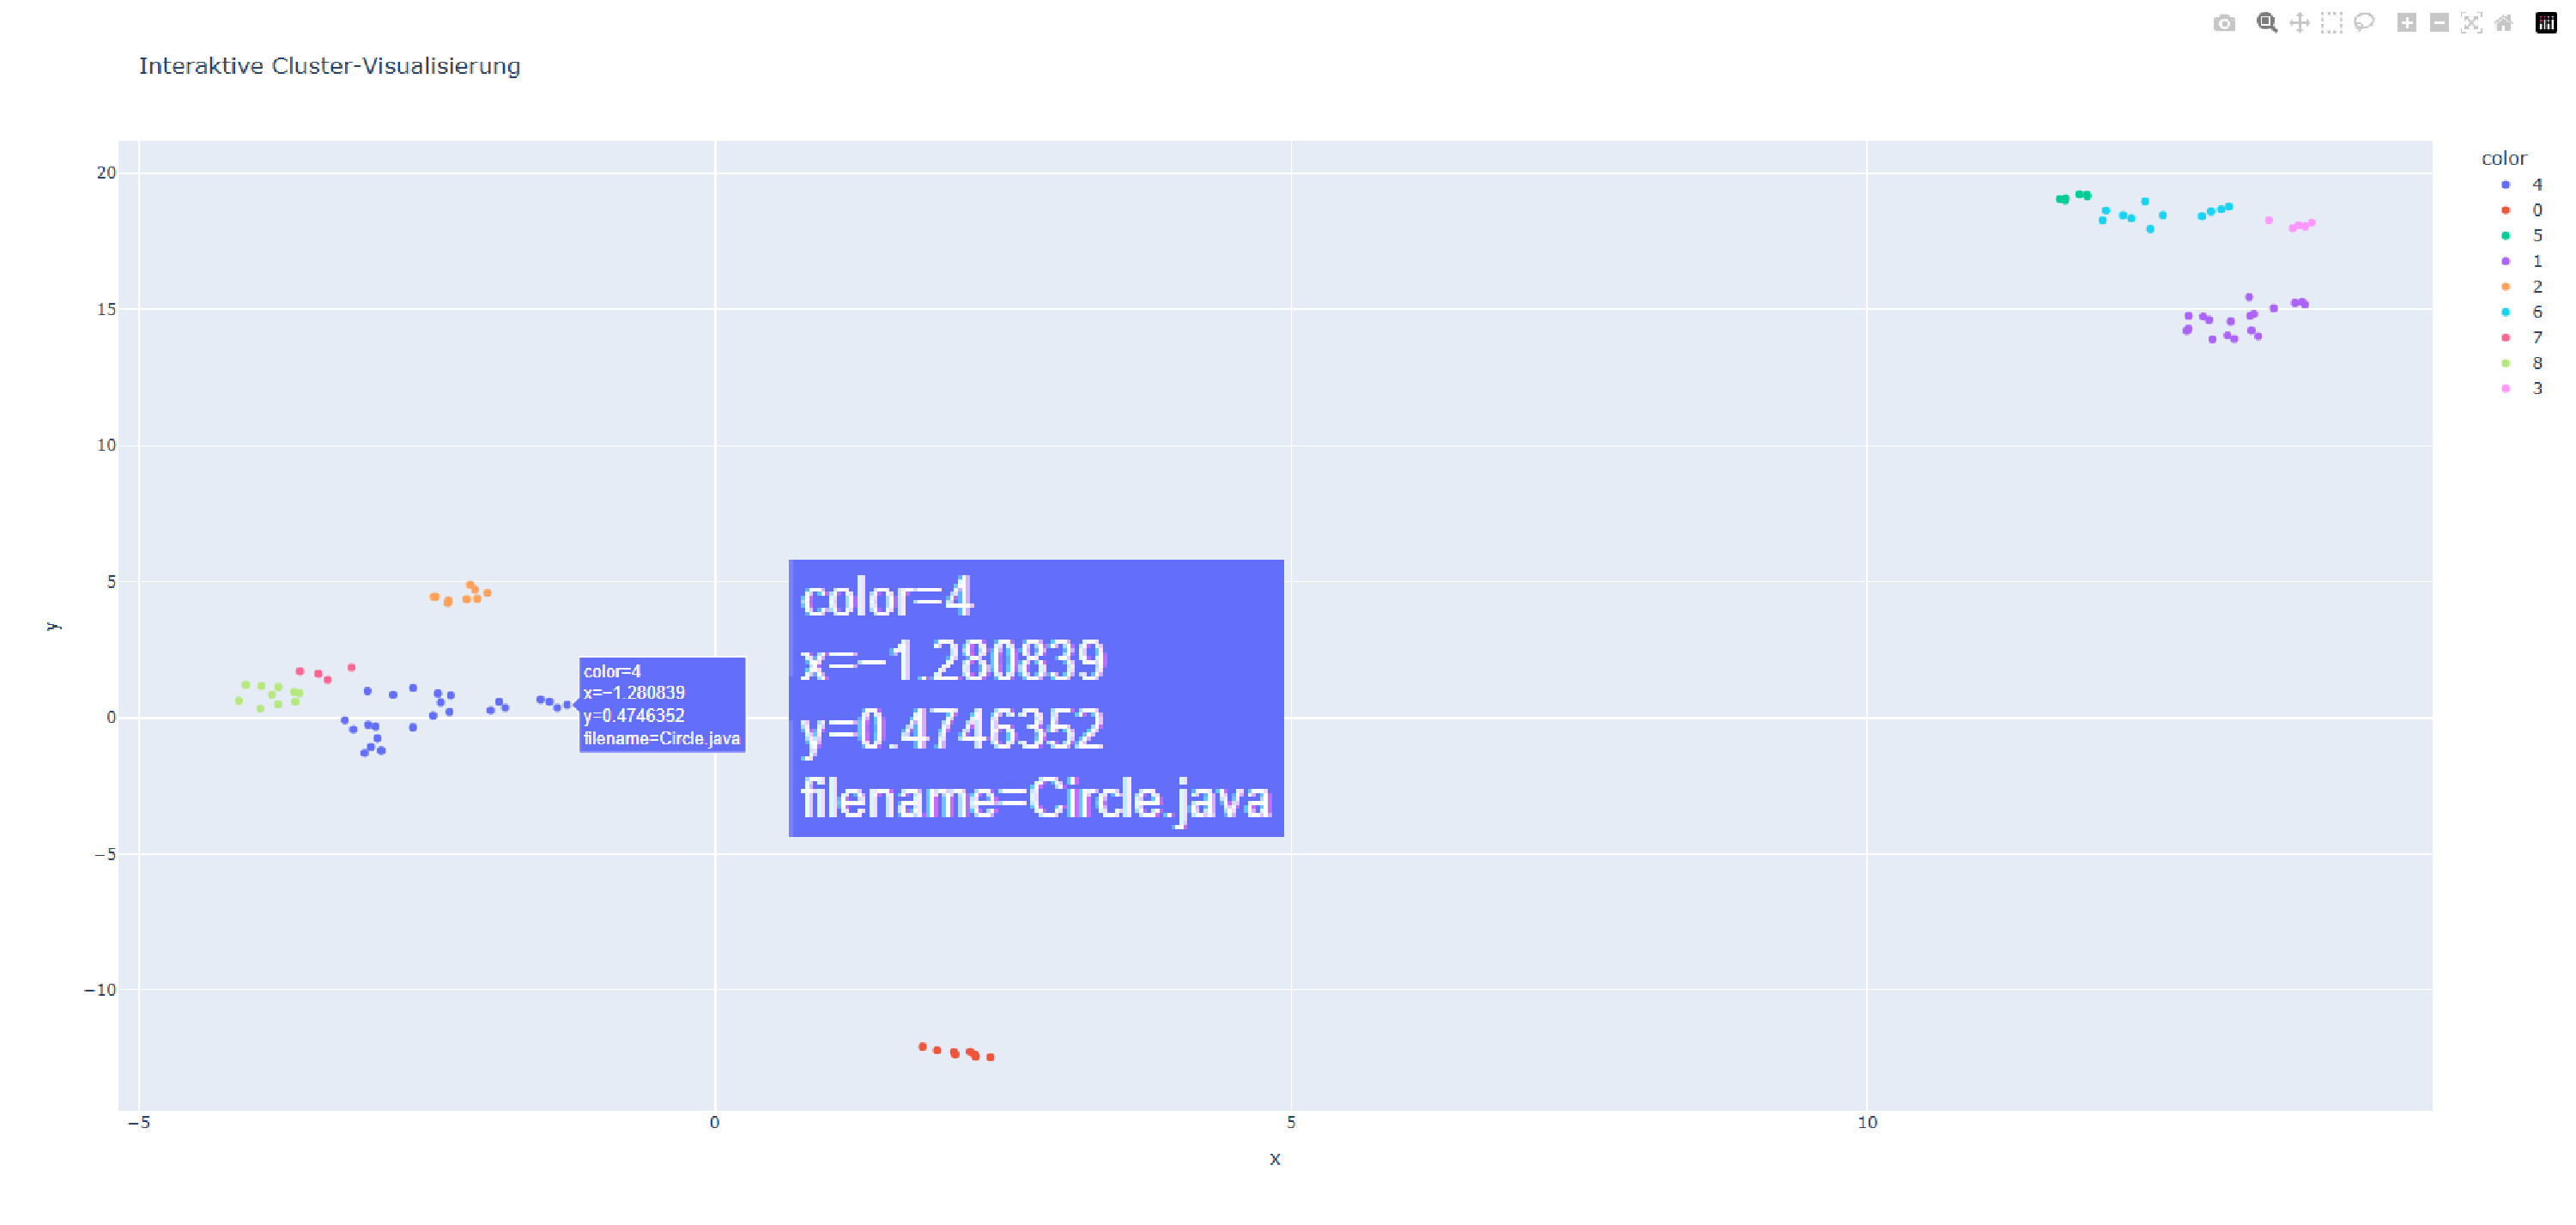
\includegraphics[width=1.0\textwidth]{images/Interaktives Clustering-Diagramm.pdf}
	\caption{Interaktives Clustering-Diagramm einer Clusterung von 147 Java-Dateien. Durch das Halten der Maus über Punkte werden Informationen über sie angezeigt (im Bild wiederholt vergrößert dargestellt). Am rechten Rand sind die Mengen der Cluster angezeigt.}
	\label{Interaktives Clustering-Diagramm}
\end{figure}

\subsection{Zweiter Implementierungsabschnitt}
In Abbildung \ref{Interaktives Clustering-Diagramm} sind zwar farbige Punkte in unterschiedlicher Anzahl pro Cluster zu erkennen, jedoch wurden keine labels angezeigt, die Informationen über die Punkte anzeigen sollten. Als vorbereitender Schritt für weiterführende Prozesse zur automatischen Feedbackgenerierung, müssen sie zumindest fürs Erste visuell zuordenbar sein. Aus diesem Grund wurde ein weiteres Modul zur Visualisierung implementiert. Das entstandene Modul \texttt{interactive\_plot.py} nahm dafür wieder Embeddings, labels und zustätzlich noch den Namen der aktuellen Java-Datei entgegen, die im \texttt{data\_loader.py}-Modul gespeichert wurden. Dazu wurden aus der Python-Bibliothek die Module Pandas\footnote{\url{https://pandas.pydata.org/docs/}} und Plotly Express\footnote{\url{https://plotly.com/python/plotly-express/}} importiert, die einerseits zur Erstellung von Tabellenstrukturen (DataFrames) und andererseits für einfache und interaktiave Plots zuständig sind. Ausgeführt, öffnete sich ein Fenster im Webbrowser mit von der Gestalung ähnlichem Plot wie in der statischen Variante (\ref{Erstes Clustering-Diagramm}).

Beim mehrmaligen Austesten verschiedener Dateimengen und Überprüfen der ausgegeben Punkte, fiel auf, dass Cluster bei größeren Datenmengen nicht mehr konsistent sind, obwohl akzeptable Ergebnisse im Evaluationsverfahren erreicht wurden. Genauer genommen wurden vereinzelt unterschiedliche Dateien in einem gemeinsamen Cluster platziert (gezeigt in \ref{abs:C-u-D-i-e-D} in Abschnitt Forschungsergebnisse). So kamen beispielsweise Point.java-Dateien in einem Cluster mit sonst nur Circle.java-Dateien vor. Da Clustering-Algorithmen nach ähnlicher Syntax und Semantik clustern, kann solch ein Verhalten durchaus vor kommen, ist hier jedoch nicht von praktischen Nutzen. Andererseits könnten ebenso Fehler in den Algorithmen oder Inkonsistenzen in den gegebenen Datensätzen die fehlerhafte Clusterung verursachen. Selbst Dateien die abhängig von der gestellten Aufgabe zu den Einreichungen bereits gegeben waren, nicht bearbeitet werden sollten und überall identisch waren, wurden in verschiedenen Clustern angeordnet. Als erste Maßnahme gegen diese Probleme, wurden die nicht zu bearbeitenden Dateien ignoriert, indem nicht mehr allgemein nach \glqq.java\grqq-Dateien gesucht wird, sondern nur noch nach bestimmten Namen. Im weiterem Verlauf wurde zudem in der pipeline eine Schleife ergänzt, die die Prozesse ab Embedding bis zur Visualisierung für die gewünschten, in der config-Datei festgelegten Namen bzw. Java-Dateien wiederholt. Dadurch werden gemischte Cluster verhindert und für jede unterschiedene Java-Datei ein Plot erstellt.
Weiterhin eim Testen einer niedriger Anzahl von Dateien (\(n \leq 4\)) ist aufgefallen, dass der Embedding-Algorithmus nicht mehr funtkioniert, jedoch ist solche eine Clusterung ohnehin nicht von Nutzen.

Um die Evaluationsverfahren einfach testen zu können, wurde eine separate experimentierungs-Pipeline erstellt. Der Vorteil bestand hierbei, dass die verschiedenen Kombinationen der Dimensionsreduktionsverfahren und Clustering-Algorithmen mit Parametern anhand dictionaries innerhalb der Pipeline definiert wurden. In den Tabellen \ref{tab:EI-EV-20} und \ref{tab:EI-EV-160} im Abschnitt Forschungsergebnisse wurde gezeigt, welche Algorithmen-Kombination für verschiedene Dateimengen geeignet sind. Die Evaluationsergebnisse wurden anschließend in einer CSV-Datei im Projektverzeichnis festgehalten.

Um den Punkten im Diagramm mehr Informationen entnehmen zu können, wurde neben den Dateinamen nun noch der Name des Ordners hinzugefügt. Da die erreichten Punktzahlen der Einreichungen Teil des Ordnernames sind, konnte jetzt die Clusterung besser nachvollzogen und überprüft werden. Weiterhin wurde das \texttt{interactive\_plot.py}-Modul um die Option das Diagramm als dreidimensionale Umgebung darzustellen erweitert. Sollten mehrere Cluster im 2D-Diagramm aufeinanderliegen, so kann durch die dritte Achse bessere Einsicht gewährleisten.

\subsection{Dritter Implementierungsabschnitt}
Auch wenn für jede durch Namen getrennte Art Datei ein separates Diagramm erstellt wird, besteht die Möglichkeit dass die vollständige Einreichung bzw. Lösung zu den gestellten Aufgaben gesamt betrachtet werden sollte, da es sonst zu verminderter Information führen könnte. Um die Dateien als ein Ganzes zu betrachten, wurde das \texttt{data\_loader.py}-Modul um eine Konkatenations-Funktionalität ergänzt. Die entstandene Methode konkateniert alle gesuchten Java-Dateien eines Einreichungsordners. Der im Diagramm gezeigte Dateiname eines Punktes, setzt sich nun aus den konkatenierten Namen zusammen. Die Schleife in der Pipeline die die Prozessschritte für jede gesuchte Art Datei wiederholte, wurde wieder entfernt.

Auch wenn das Programm in der Lage ist die Embeddings ohne Dimensionsreduktionsverfahren zu behandeln um sie für weiterführende Projekte vorzubereiten bzw. zu clustern, ist es zum Testen immer noch mehr geeignet sie sinnvoll visuell anzeigen zu können. Daneben ist durch die Anzeige der Ordnernamen pro Punkt ein weiters Problem aufgefallen. So werden konkatenierte Dateien in einen Cluster gesteckt, dessen Ordnernamen sich durch stark variierende Punktzahlen unterscheiden, wie in Abbildung \ref{a1} gezeigt.